\documentclass{report}

% PACKAGES
\usepackage[margin=1.00in]{geometry}
\usepackage[pdftex]{graphicx}
\usepackage[table,xcdraw]{xcolor}
\usepackage{indentfirst}
\usepackage{caption}
\usepackage{float}
\usepackage{caption}
\usepackage{subcaption}

% \usepackage{natbib}

\bibliographystyle{ieeetr}

\usepackage{Sweave}
\begin{document}
\Sconcordance{concordance:upstat_report.tex:upstat_report.Rnw:%
1 12 1 1 0 23 1 1 25 45 1 1 23 1 2 26 1 1 22 1 2 24 1 1 91 1 23 1 2 24 %
1 1 15 1 2 15 1 1 10 1 2 9 1 1 88 1 2 29 1}

\begin{titlepage}

\begin{center}

~\\[4cm]

\textsc{\Large Culver Road and East Main Street Intersection}\\[1.5cm]
\textsc{\huge Traffic Analysis Report}\\[8.5cm]



\vfill

{ March 20, 2015}

\end{center}
\end{titlepage}

\noindent
\section*{Introduction}

%This subsection should include a diagram of the interesction and some statistics
%about the interection. This should include information about the traffic flow
%rate (volume), the LOC classification, and some general information that is
%useful to the DOT.

There has been intense study in the area of traffic management since the mid-1990s. The ability to quantify and discern underlying patterns with a simple loop detector is a useful tool in understanding the complex nature of transportation systems. We were tasked with identifying unique trends present in data from a magnetic loop sensor and to provide sound recommendations to improve traffic conditions for the intersection of Culver Road and East Main Street in Rochester, New York. The data, obtained from a loop detector approximately 200 feet away from intersection in the southbound lane, has nearly eight months of data stretching from October of 2013 to June of 2014. The loop detector transmits data in five minute intervals, and calculates pertinent metrics such as estimated hourly volume, number of vehicles approaching a red light, delay, and the speed of the vehicles as they approach the intersection.

The intersection, pictured in Figure \ref{fig:intersection}, is part of an important byway between Bay Street and East Main Street. Zoning data provided by the city of Rochester shows us that the area surrounding this portion of Culver Road is mainly residential. However, there are designated commercial zones at both the intersections of Bay and East Main, and additional commercial lots in between both of these locations \cite{PropInfo}. These are mainly smaller business and not large scale commercial plazas similar to those in Henrietta or elsewhere in the city of Rochester. It is important to consider this information in conjunction with the results of our analyses when providing meaningful suggestions.

We also used the Traffic Volume Map that is provided by the Monroe County and the City of Rochester. Culver Road normally experiences a large amount of traffic that is comparable to East Main \cite{TrafficMap}. Furthermore, it appears as though the traffic continues down Culver and that there is no noticeable amount of traffic turning onto East Main that would contribute to any possible congestion.

\begin{figure}[H]
        \centering
        \begin{subfigure}[b]{0.45\textwidth}
                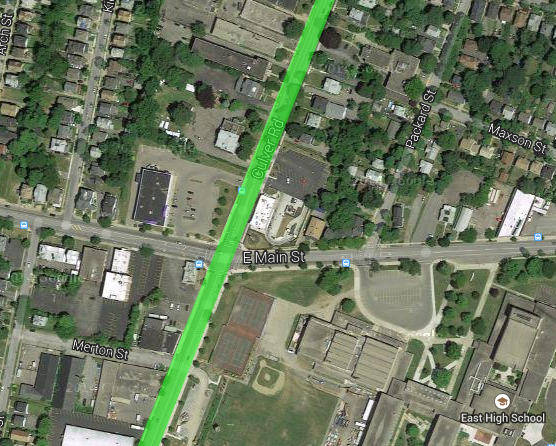
\includegraphics[width=\textwidth]{satellite_H.png}
        \end{subfigure}
        \begin{subfigure}[b]{0.45\textwidth}
                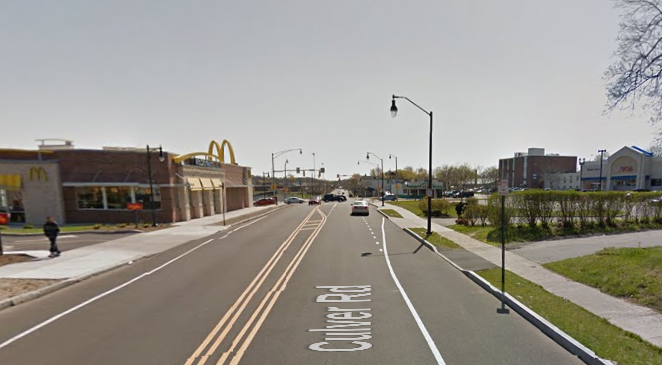
\includegraphics[width=\textwidth]{streetview.png}
        \end{subfigure}
        \caption{Pictured Left: satellite image of the intersection of Culver and East Main. Culver Road is highlighted in a light green. To the bottom right is East High School of the Rochester School District. Pictured Right: A streetview of Culver Road as it approaches East Main. Several businesses are located on both sides of the street. Location is approximate to where the loop detector is installed. Both images courtesy of Google Maps.}
        \label{fig:intersection}
\end{figure}

\noindent
\section*{Data Analysis}

To assess the traffic conditions at the Culver Road and East Main Street
intersection, we determined the current state of the intersection in terms of
federal DOT guidelines for this class of intersection, as well as analyses to
examine trends and patterns in the traffic recorded, and the calculation of the
probability of traffic congestion based on the time of day and day of the week.


\subsection*{Traffic Analysis}

There are a few common characteristics to examine when determining the traffic
flow for a particular intersection. Namely, it is important to determine the
amount of delay experienced by drivers as they enter the intersection, the density
of the vehicles as they pass through the intersection, and the velocity at which
traffic flows through the intersection. With these three variables, it is possible
to determine the conditions that result in congestion at this intersection.

The amount of time that vehicles wait at an intersection is referred to as the
Level of Service (LOS). Ranked in letter grades from A to F, the LOS is an
identifier for the overall health of the intersection. Ideally, an intersection
should be classified as being either A, B, or C, denoting free flow, reasonably
free flow, and stable flow, respectively. The 2010 Highway Capacity
Manual classifications for LOS can be seen in Table \ref{LOStable}, in which grade
A intersections have less then 10 seconds of vehicle control delay, whereas grade
F intersections have more than 80 of vehicle control delay.

\begin{table}[h]
\centering
\caption{Level of Service classifications published in the 2010 Highway Capacity
Manual.}
\begin{tabular}{c | c}
\textbf{LOS} & \textbf{Vehicle Control Delay (Sec.)}\\\hline
A & $\le 10$\\
B & $10 - 20 $\\
C & $20 - 35$\\
D & $35 - 55$\\
E & $55 - 80$\\
F & $\ge 80$\\
\end{tabular}
\label{LOStable}
\end{table}

Using these classifications, we examined the average vehicle control delay for
each five minute observation period. As shown in Figure \ref{fig:LOSfigure},
the majority of observations have a Grade F Level of Service (58.38\%). Each of
the other levels of service occurred in between 7.45\% and 8.63\% of observations.
This suggests that the Culver Road and East Main Street intersections is
experiencing traffic congestion, in which each vehicle move in lock step with
the vehicle in front of it \cite{HCM}.

\begin{figure}[h]
\centering
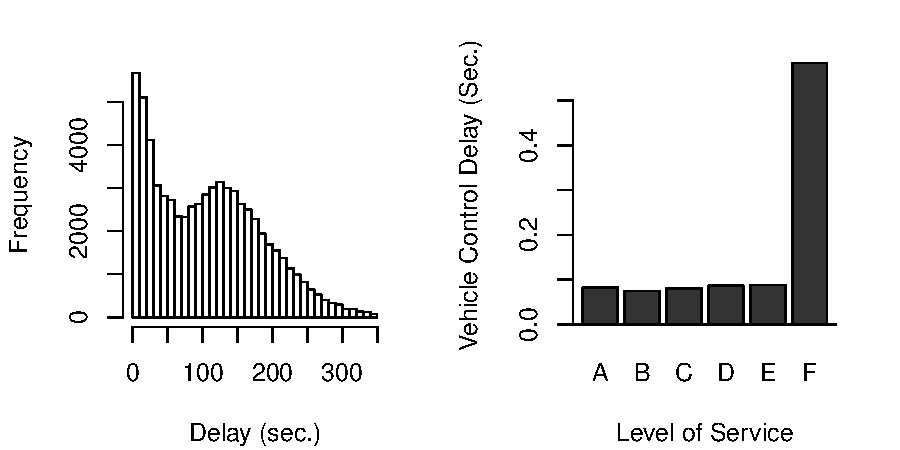
\includegraphics{upstat_report-LOCplot}
\caption{The Culver Road/East Main Street
intersection has a poor Level of Service. The histogram on the left shows the
distribution of the average vehicle control delay for each observation. The
distribution is bimodal with peaks at zero seconds and 140 seconds. The median
delay was 103 seconds with a IQR of
123 seconds. The bar plot on the right shows the
distribution of each LOS grade for each observation in our data set.
Observations were given a letter grade based on the average vehicle control
delay for each 5 minute interval. The majority of all observations had a delay
of greater than 80 seconds, suggesting that the intersection is predominantly grade
F.}
\label{fig:LOSfigure}
\end{figure}

We also examined the relationship between the traffic density and traffic volume,
also known as flux. When plotted, the relationship between the traffic density
and the traffic volume creates the fundamental diagram of traffic flow
\cite{HCM}, as shown in Figure \ref{fig:Fundamental}. Using linear regression techniques, we
were able to estimate the free flow velocity to be 19.5 miles per hour and the
traffic wave velocity to be 2.43 miles per hour against the direction of traffic.
We also determined the critical traffic density to be 42.8 vehicles per mile.
As the vehicle density passes the critical density, the traffic flow becomes
more unstable leading to traffic waves and congestion. To maximize
the traffic flow, the vehicle density must remain below the critical density.

\begin{figure}[h]
\centering
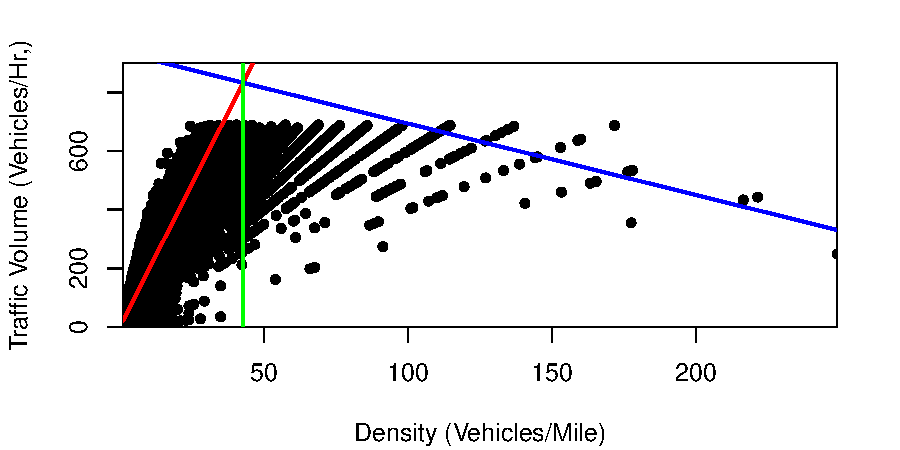
\includegraphics{upstat_report-003}
\caption{Fundamental diagram of traffic flow provides
free flow and traffic wave velocities. Traffic density was calculated by
dividing the traffic volume by the traffic speed. Using linear regression, we
found the free flow velocity (19.5 mph) as depicted in red, the traffic wave
velocity (2.43 mph) as depicted in blue, and the critical density (42.8 vehicles
per mile) as depicted in green.}
\label{fig:Fundamental}
\end{figure}


\subsection*{Trend Analysis}

To examine general trends from the metrics we were provided, we performed linear
regression on the traffic delay and the traffic volume. This techniques allows
us to approximate the traffic volume and delay over multiple observations.
Figure \ref{trends} shows the median delay for each week and
the median traffic volume for each week with the linear regression for each data
set. Our data suggest that the median amount of time that vehicles wait at the
intersection may be increasing by 0.24 seconds per week. Our data also suggest
that the median number of vehicles utilizing the intersection may be increasing
by approximately 11 vehicles per week. Although the correlation coefficients are
rather low, we are confident that the traffic congestions will worsen as more
vehicles utilize the intersection.

\begin{figure}[H]
\centering

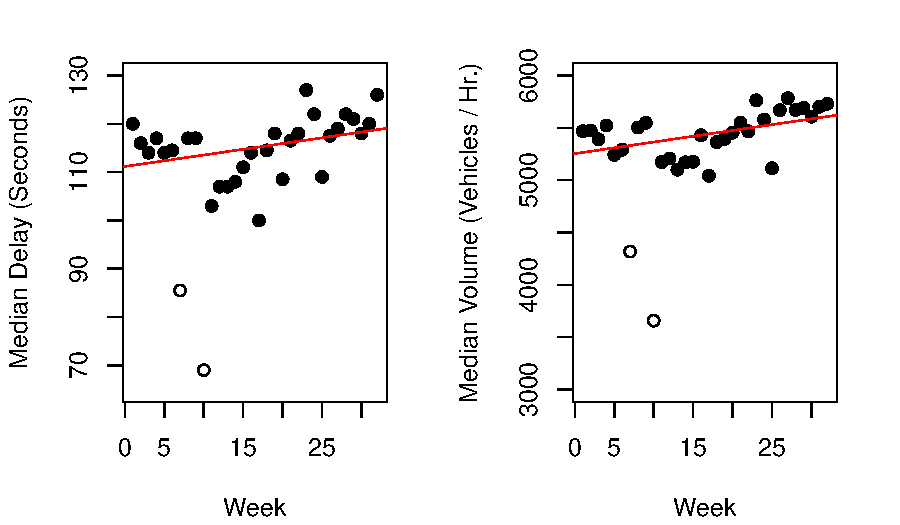
\includegraphics{upstat_report-VolumePlot}
\caption{The median traffic delay and median weekly
traffic volume are increasing over time. A linear regression of the median
traffic delay for each week suggests that the traffic delay may be increasing
0.24 seconds per week
($R^2 = 0.13$). Similarly, a linear
regression of the median number of vehicles to pass through the intersection per
week suggests that the number of vehicles utilizing the intersection may be
increasing at a rate of 11.08 vehicles
per week ($R^2 = 0.24$).}
\label{trends}
\end{figure}

\subsection*{Pattern Analyses}

A secondary way of understanding the traffic passing though the Culver Road and
East Main Street intersection is to assess the prevailing patterns of traffic.
Two methods of analyzing traffic patterns are clustering and correlation analysis.
Clustering algorithms give us an opportunity to treat each day's traffic like
a single data point. By comparing the distance between each day's traffic, we can
group similar traffic patterns together. Correlation analyses, on the other hand,
examine how similar each individual pairing of days is by comparing each traffic
5-minute observation. These two different techniques provide different ways of
finding patterns: clustering allows us to find similar large-scale similarities
between days, whereas correlations gives a more granular measure of similarity
between a day and the expected traffic.

Using a CLARA clustering algorithm, we clustered the daily traffic volume
for each day of data using 10-minute intervals. We found that there are three
primary types of traffic: weekday traffic, Saturday traffic, and Sunday traffic.
Each of these types is named after the days in which they are most likely to
occur. Figure \ref{fig:clustering}A, shows a cluster plot of the three clusters
of traffic measured along their principle components. The gray circles represent
traffic classified as Sunday traffic, the orange triangles are weekday traffic, and
the blue pluses are Saturday traffic. It should be noted that the most variable traffic
type is the Sunday classification, suggesting that there may be incidences of
highly irregular traffic that are more similar to Sundays than any other day
of the week. A notable example of this is Thanksgiving Thursday on November 28,
2013. Thanksgiving experiences drastically lower traffic than both the typical
Sunday and the typical Thursday, but the low traffic volume is more similar to
a Sunday so it was clustered accordingly, as shown in Figure \ref{fig:clustering}B.

\begin{figure}[H]
\centering
\begin{subfigure}[b]{0.45\textwidth}
\centering
A\\
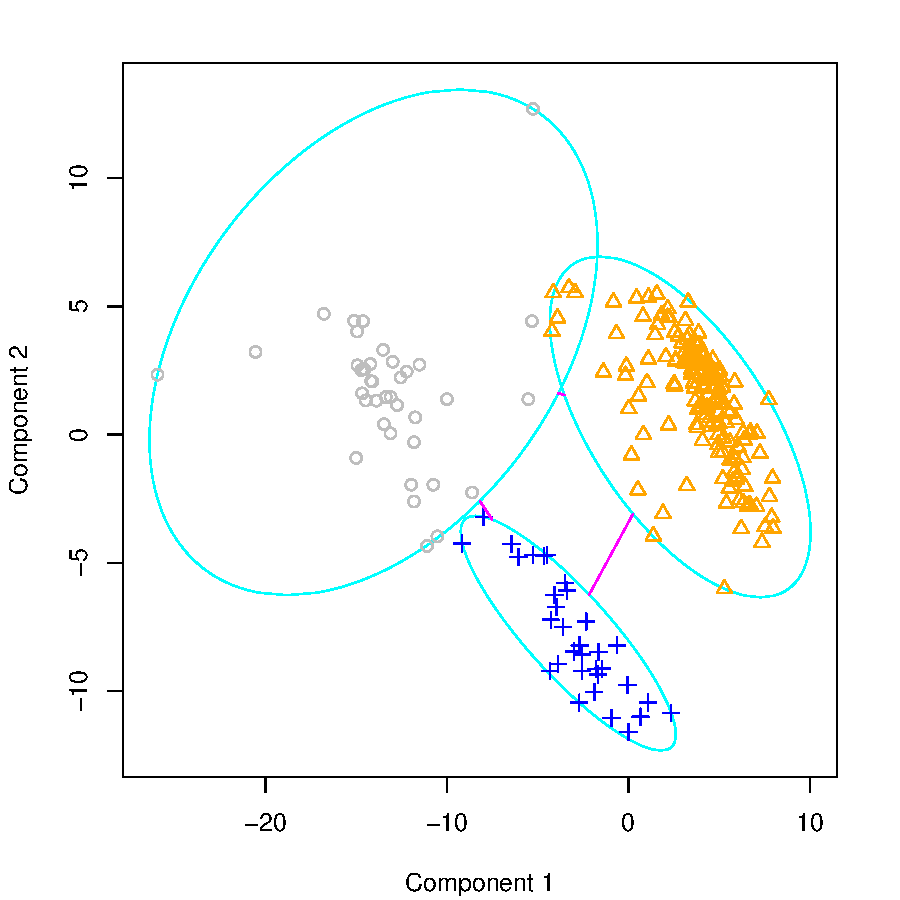
\includegraphics{upstat_report-clustering}
\end{subfigure}
\begin{subfigure}[b]{0.45\textwidth}
\centering
B\\
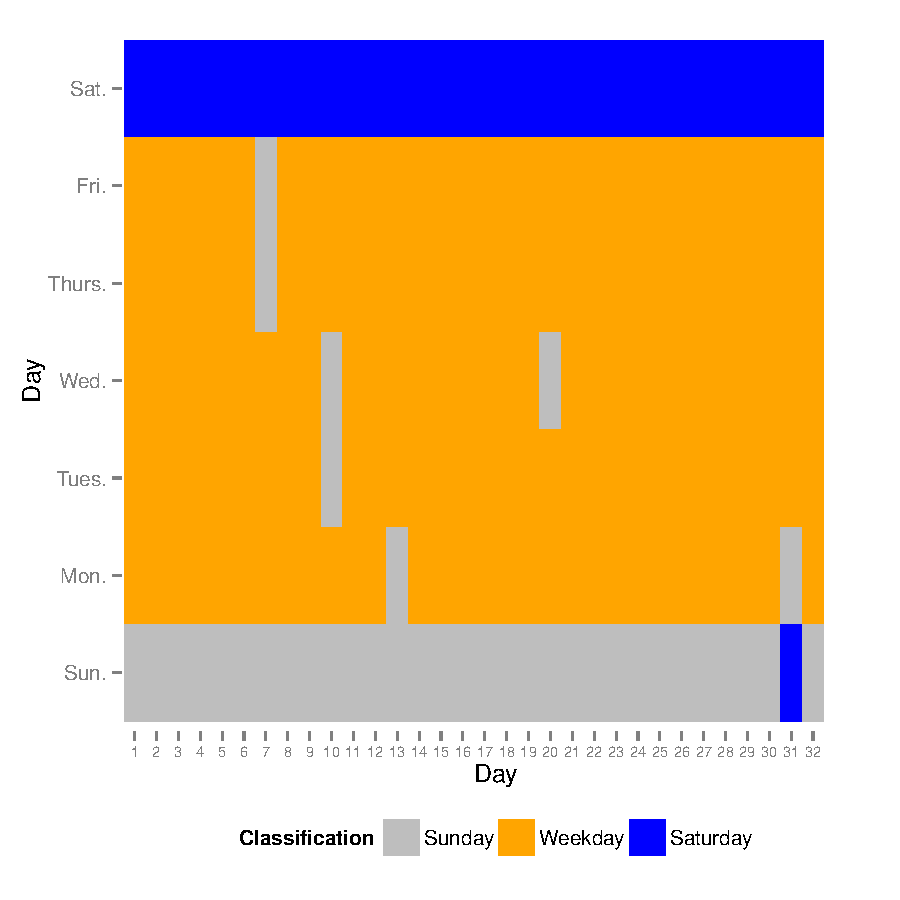
\includegraphics{upstat_report-007}
\end{subfigure}
\caption{CLARA clustering suggests three primary traffic types. Each day's traffic volume
was aligned in a matrix and clustered using a CLARA clustering algorithm. Subfigure A shows a plot of the principle components of the days clustered. Similar traffic types are grouped spatially together in a manner that allows them to be clustered easily. Figure B shows a calendar view of each day as classified by the CLARA clustering algorithm. This plot clearly shows the weekly relationship between the traffic types, and highlights traffic abnormalities.}
\label{fig:clustering}
\end{figure}


For our correlation analysis we compared each day's traffic volume to the median
traffic for that day of the week. For example, we examined the correlation between
the traffic volume for Thanksgiving to the median traffic volume at each 5-minute
interval for all Thursdays. A plot of each day's correlation, as shown in Figure \ref{fig:correlation},
outlines the variability in each day's traffic patterns. It should be noted that
the days of abnormally low correlation relate to weekdays clustered as Sunday
traffic in Figure \ref{fig:clustering}B. In this figure, high correlation suggests that
the day's traffic is very similar to the expected traffic for that day of the week,
whereas a low correlation is indicative of an abnormality in traffic volume.
One interesting case of abnormal traffic is the seventh Thursday of the data set,
which corresponds to Thanksgiving. The 2013 Thanksgiving traffic was abnormally
low for a Thursday. Similarly, the 10th and 20th Wednesdays of the data set
exhibit similar patterns of minimal traffic. Interestingly, weekdays have a higher
median correlation (0.946) and a lower
variance in correlation (0.003) than the weekends. This
suggests that weekdays have a relatively stable or predictable traffic pattern
with a few dramatic exceptions.

\begin{figure}[h]
\centering
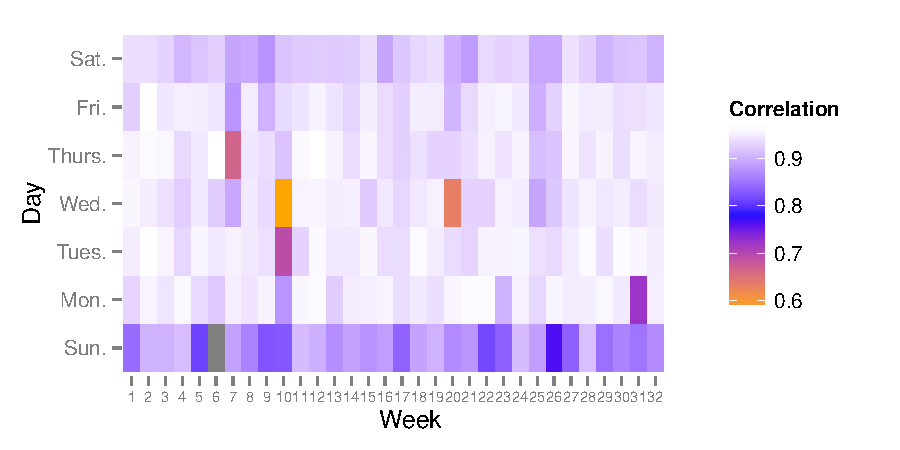
\includegraphics{upstat_report-008}
\caption{Correlation analysis shows holidays, data collection errors, and small-scale
traffic patterns. In this color scale, white indicates high correlation, purple
indicates moderate correlation, and orange indicates low correlation. Some days of
interest include the seventh Thursday, which corresponds with Thanksgiving, the
10th Tuesday and Wednesday, and the 20th Wednesday.}
\label{fig:correlation}
\end{figure}


\subsection*{Bayesian Analysis}

In order to determine how the probability of congestion relates to the time of day we adapted Bayes' Theorem for use with the data provided. Because the traffic on the weekend is not as intense as the traffic during the weekdays, the decision was made to evaluate each day independently of one another so as not to induce any sort of bias into the results. Congestion was determined simply by using the critical density of the intersection, identified as 42.8 Vehicles per Mile. Any situation where the density is equal to or greater than this measure is determined to be 'congested.' Any situation below this measure is simply 'not congested.'

This is then sorted for each time step, and a proportion is generated about how many times (on a specific day of the week) that particular time is considered congested. For example, this means that if 2 out of the 10 observations at 2:10am on Wednesdays is considered to be congested, equal or exceeding the critical density, the proportion is calculated to be 0.2. This is then multiplied by the probability of congestion at any time amongst all the observations, and is then divided by the probability of randomly selecting that time from the dataset.

Figure \ref{bayesplot} provides a way of seeing the probability of congestion
occurring given the day of the week and the time of day. As expected the probability
of congestion increases dramatically between 4 and 6 PM, which correspond with the
traditional rush hour period. Interestingly, there is a non-trivial probability of
traffic congestion occurring between 2 and 6 AM. This may correspond with people
who work during the evening. Additionally, there is a slight spike at 7 AM, which
may correspond with school traffic or people leaving for jobs with 7:20 or 8 AM
starting times.

\begin{figure}[h] \label{bayesplot}
\centering
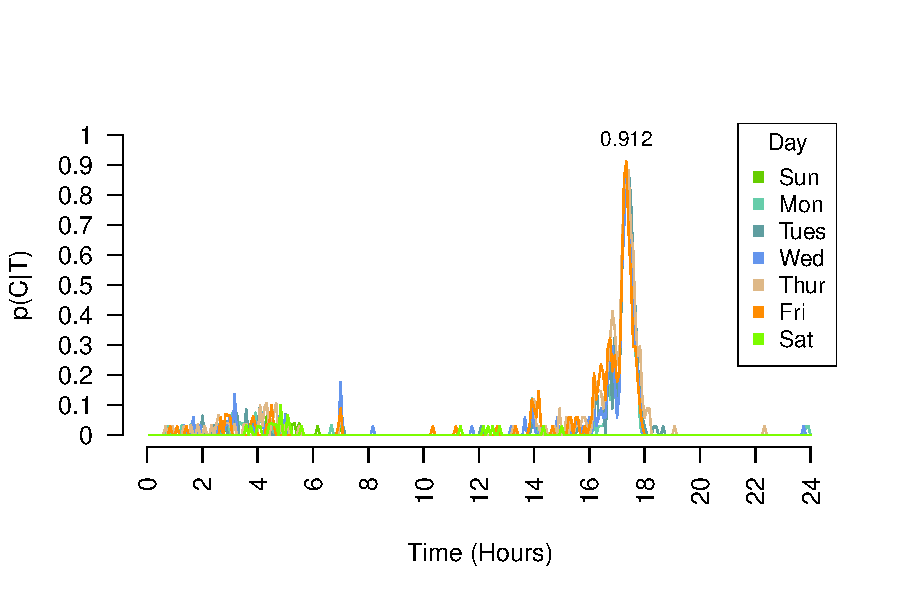
\includegraphics{upstat_report-bayesplot}
\caption{Probability of observing congestion based on specific times throughout the day (represented as p(C|T)). All days are represented as separate lines. A maximum probability of 91.2\% is shown on the graph and occurs at 5:15pm on Friday. Most weekdays have the highest probability of congestion between 5:00pm and 5:25pm, or during evening rush hour.}
\end{figure}

Table \label{basestable} presents times that have he highest probability of observing traffic congestion. For the purposes of this table Saturday and Sunday were omitted from the table due to the fact that their relative probabilities were approximately zero. A point of interest
is that congested periods start earlier on Fridays, suggesting that people may
be leaving work early on Fridays.

\begin{table}[h] \label{bayestable}
\centering
\caption{Selected results from Bayesian analysis of traffic data.}
\begin{tabular}{l|l
>{\columncolor[HTML]{EFEFEF}}l l
>{\columncolor[HTML]{EFEFEF}}l l}
\textbf{Time} & \textbf{Mon} & \textbf{Tues}                & \textbf{Wed} & \textbf{Thur} & \textbf{Fri}                                         \\ \hline
17:05         & 0.500          & 0.471                        & 0.529        & 0.588         & \cellcolor[HTML]{FFFFFF}0.500                          \\
17:10         & 0.765        & 0.824                        & 0.677        & 0.824         & \cellcolor[HTML]{FFFFFF}{\color[HTML]{333333} 0.853} \\
17:15         & 0.824        & {\color[HTML]{333333} 0.853} & 0.882        & 0.824         & 0.912                                                \\
17:20         & 0.853        & 0.882                        & 0.765        & 0.882         & 0.677                                                \\
17:25         & 0.588        & 0.794                        & 0.647        & 0.677         & 0.529
\end{tabular}
\end{table}


\noindent\section*{Recommendations}

Culver Road is an important byway for the citizens of Rochester, and it's ability to function properly is critical in order to avoid unnecessary congestion whenever possible. Considering that the intersection has a Grade F LOS approximately sixty percent of the time, appropriate action must be taken in order to reduce the amount of time vehicles are waiting at this intersection. Since both East Main and Culver are high volume roads, an alteration of the intersection signal light to allow more traffic to flow through the intersection via Culver would most most likely cause more harm than good.
Similarly, the speed at which cars enter the intersection is a function of the traffic at the intersection it self, so altering the speed of Culver Road will not relieve traffic.

Instead, we offer four potential solutions that could reduce the incidence of traffic congestion. Based on the published traffic volume maps and the recorded data, Culver experiences more north-south traffic than turning traffic, we suggest that Culver be widened into a two lane avenue so that it can accommodate the higher amount of traffic moving from north to south. Widening Culver would have a dramatic effect on reducing the amount of time vehicles are waiting at the intersection and thereby increasing the LOS.A second infrastructure change that could reduce traffic congestion is the lengthening of turn lanes. In the case that there is an up tick in turning traffic, turning vehicles can extend past the designated lane and disrupt the south-bound majority.

A non-infrastructure suggestion is to limit the number of commercial permits and to rezone available lots to be residential-only. Our data suggest that there is a surge in volume during the typical "end of the work day." This is also supported by our Bayesian analysis of congestion probability. Should we have access to data for the north bound lane of Culver at this intersection it would be likely that we would see high volume in the morning. These vehicles could simply be representative of individuals commuting to work, and by reducing the number of businesses in the area, you could thereby reduce traffic and eliminate the need to increase the capacity of the road itself.

Our last recommendation is the formation of an automated system to classify traffic on-the-fly. Such a system would be able to diagnose abnormal traffic patterns and predict whether a given day is experiencing abnormally high or low traffic. This would provide the Monroe County Department of Transportation an early warning about traffic collisions, signal timing malfunctions, or other issues that may affect drivers.

In conclusion, we have shown that the current traffic conditions at the intersection of Culver Road and East Main Steet are untenable and require remediation. While this report is by no means comprehensive, it does present a stark image of increasing traffic congestion as the traffic volume and delay times increase week by week. Regardless of the solutions implemented, it is important that the traffic density at this intersection be reduced and the traffic congestion relieved while it is still feasible to do so.

\begin{thebibliography}{9}
  \bibitem{PropInfo}
    City of Rochester,
    \emph{Property Information Application}.
    HTTP://maps.cityofrochester.gov/propinfo/.
  \bibitem{TrafficMap}
    City of Rochester,
    \emph{Traffic Volume Map}.
    2014.
    http://www2.monroecounty.gov/files/dot/pdfs/City-adt-map-through-2014.pdf.
  \bibitem{HCM}
    Transportation Research Board of the National Academies,
    \emph{Highway Capacity Manual 2010}.
    5th edition,
    2010.
\end{thebibliography}

\end{document}
